\documentclass{beamer}
\usepackage[utf8]{inputenc}

\usetheme{Madrid}
\usecolortheme{default}
\usepackage{amsmath,amssymb,amsfonts,amsthm}
\usepackage{txfonts}
\usepackage{tkz-euclide}
\usepackage{listings}
\usepackage{adjustbox}
\usepackage{array}
\usepackage{tabularx}
\usepackage{gvv}
\usepackage{lmodern}
\usepackage{circuitikz}
\usepackage{tikz}
\usepackage{graphicx}

\setbeamertemplate{page number in head/foot}[totalframenumber]

\usepackage{tcolorbox}
\tcbuselibrary{minted,breakable,xparse,skins}



\definecolor{bg}{gray}{0.95}
\DeclareTCBListing{mintedbox}{O{}m!O{}}{%
  breakable=true,
  listing engine=minted,
  listing only,
  minted language=#2,
  minted style=default,
  minted options={%
    linenos,
    gobble=0,
    breaklines=true,
    breakafter=,,
    fontsize=\small,
    numbersep=8pt,
    #1},
  boxsep=0pt,
  left skip=0pt,
  right skip=0pt,
  left=25pt,
  right=0pt,
  top=3pt,
  bottom=3pt,
  arc=5pt,
  leftrule=0pt,
  rightrule=0pt,
  bottomrule=2pt,
  toprule=2pt,
  colback=bg,
  colframe=orange!70,
  enhanced,
  overlay={%
    \begin{tcbclipinterior}
    \fill[orange!20!white] (frame.south west) rectangle ([xshift=20pt]frame.north west);
    \end{tcbclipinterior}},
  #3,
}
\lstset{
    language=C,
    basicstyle=\ttfamily\small,
    keywordstyle=\color{blue},
    stringstyle=\color{orange},
    commentstyle=\color{green!60!black},
    numbers=left,
    numberstyle=\tiny\color{gray},
    breaklines=true,
    showstringspaces=false,
}
\title{4.7.43}
\date{12th September, 2025}
\author{Puni Aditya - EE25BTECH11046}

\begin{document}

\frame{\titlepage}
\begin{frame}{Question}
Show that the points $\brak{\hat{i}-\hat{j}+3\hat{k}}$ and $3\brak{\hat{i}+\hat{j}+\hat{k}}$ are equidistant from the plane $\vec{r}\cdot\brak{5\hat{i}+2\hat{j}-7\hat{k}} + 9 = 0$ and lie on opposite sides of it.
\end{frame}

\begin{frame}{Theoretical Solution}
Let the given points be $\vec{P_1} = \myvec{1 \\ -1 \\ 3}$ and $\vec{P_2} = \myvec{3 \\ 3 \\ 3}$.
The equation of the given plane is
\begin{align}
    \myvec{5 & 2 & -7}\vec{x} + 9 = 0
\end{align}
This can be written in the standard form $\vec{n}^\top\vec{x} = k$. Here, $\vec{n} = \myvec{5 \\ 2 \\ -7}$ and $k = -9$.
\begin{align}
    \myvec{5 & 2 & -7}\vec{x} = -9 \label{eq:plane_eqn}
\end{align}
\end{frame}

\begin{frame}{Theoretical Solution}
The reflection of point $\vec{Q}$ with respect to the plane $\vec{n}^\top\vec{x}=k$ is given by
\begin{align}
    \vec{R} = \vec{Q} - \frac{2\brak{\vec{n}^\top\vec{Q}-k}}{\norm{\vec{n}}^2}\vec{n}
\end{align}

Let the reflection of point $\vec{P_1}$ with respect to the plane be $\vec{Q}$.
\begin{align}
    \vec{Q} &= \vec{P_1} - \frac{2\brak{\vec{n}^\top\vec{P_1}-k}}{\norm{\vec{n}}^2}\vec{n} \\
    &= \myvec{1 \\ -1 \\ 3} - \frac{-18}{78}\myvec{5 \\ 2 \\ -7} \\
    &= \myvec{\frac{28}{13} \\ -\frac{7}{13} \\ \frac{18}{13}}
\end{align}
\end{frame}

\begin{frame}{Theoretical Solution}
Let a plane parallel to given plane pass through $\vec{P_1}$. Let this be $\vec{n}^\top\vec{x}=c$
\begin{align}
    \vec{n}^\top\vec{Q} &= c \\
    \myvec{5 & 2 & -7}\myvec{\frac{28}{13} \\ -\frac{7}{13} \\ \frac{18}{13}} &= c \\
    c &= \frac{140}{13}-\frac{14}{13}-\frac{126}{13} \\
    c &= 0
\end{align}
\end{frame}

\begin{frame}{Theoretical Solution}
\begin{align}
    \vec{n}^\top\vec{P_2} &= \myvec{5 & 2 & -7}\myvec{3 \\ 3 \\ 3} \\
    &= 15+6-21 \\
    &= 0 = c
\end{align}

$\because \vec{P_2}\text{ lies in the plane }\vec{n}^\top\vec{x}=c$, the point $\vec{P_2}$ and $\vec{P_1}$ are equidistant from the plane $\vec{n}^\top\vec{x} = k$ and lie on the opposite sides of the plane.
\end{frame}

\begin{frame}{Plot}
    \begin{figure}
        \centering
        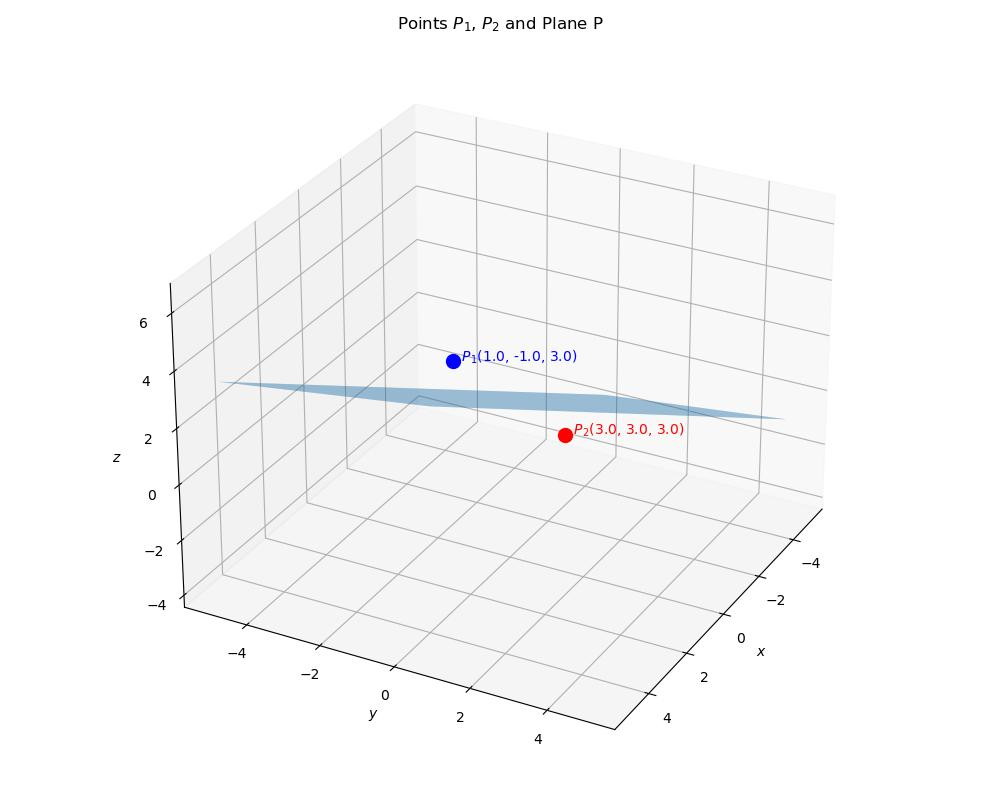
\includegraphics[width=0.5\columnwidth]{../figs/plot_c.jpg}
        \caption{Plot}
        \label{fig:fig}
    \end{figure}
\end{frame}

\end{document}
